\chapter{性能测试与结果分析}

\section{实验环境配置}

本段将简单介绍运行Plasma的必要环境配置。这包括进行性能测试的集群硬件配置,以及编译、运行Plasma所需的其他软件要求。

\subsection{天河高性能集群硬件简介}

运行测试的天河高性能集群有超过100台CPU服务器,并由100GB的Infiniband高速网络连接而成。每个CPU节点的关键配置如下所示:

\begin{table}[h]
    \centering
    \caption{天河CPU服务器硬件配置}
    \begin{tabular}{*{4}{c}}
        \toprule
        硬件组件  & 数量 & 硬件型号 & 参数配置 \\
        \midrule
        CPU  	 & 2  & Intel(R) Xeon(R) Gold 6150 & \makecell{18核 @2.7GHz \\ L1 Cache 64K \\ L2 Cache 1024K \\ L3 Cache 25344K} \\
        \midrule
        内存 	 & 12 & / & \makecell{16Gb DDR4 \\ with ECC} \\
        \midrule
    	以太网卡 & 1  & Mellanox MT27710 Family [ConnectX-4 Lx]   & 25Gb/s \\
    	IB网卡   & 1  & Mellanox MT27700 Family [ConnectX-4] & 100Gb/s \\
        \bottomrule
    \end{tabular}
    \label{tab:hardware_config}
\end{table}

每个CPU服务器配备有双路Intel至强金牌处理器。每个CPU为6通道16G内存,因此每节点内存总量为192Gb。两路处理器形成两个NUMA节点,每节点上分别挂载有一张网卡。
该型服务器的硬件拓扑图如\autoref{fig:server_block}所示。

\begin{figure}[h]
	\centering
	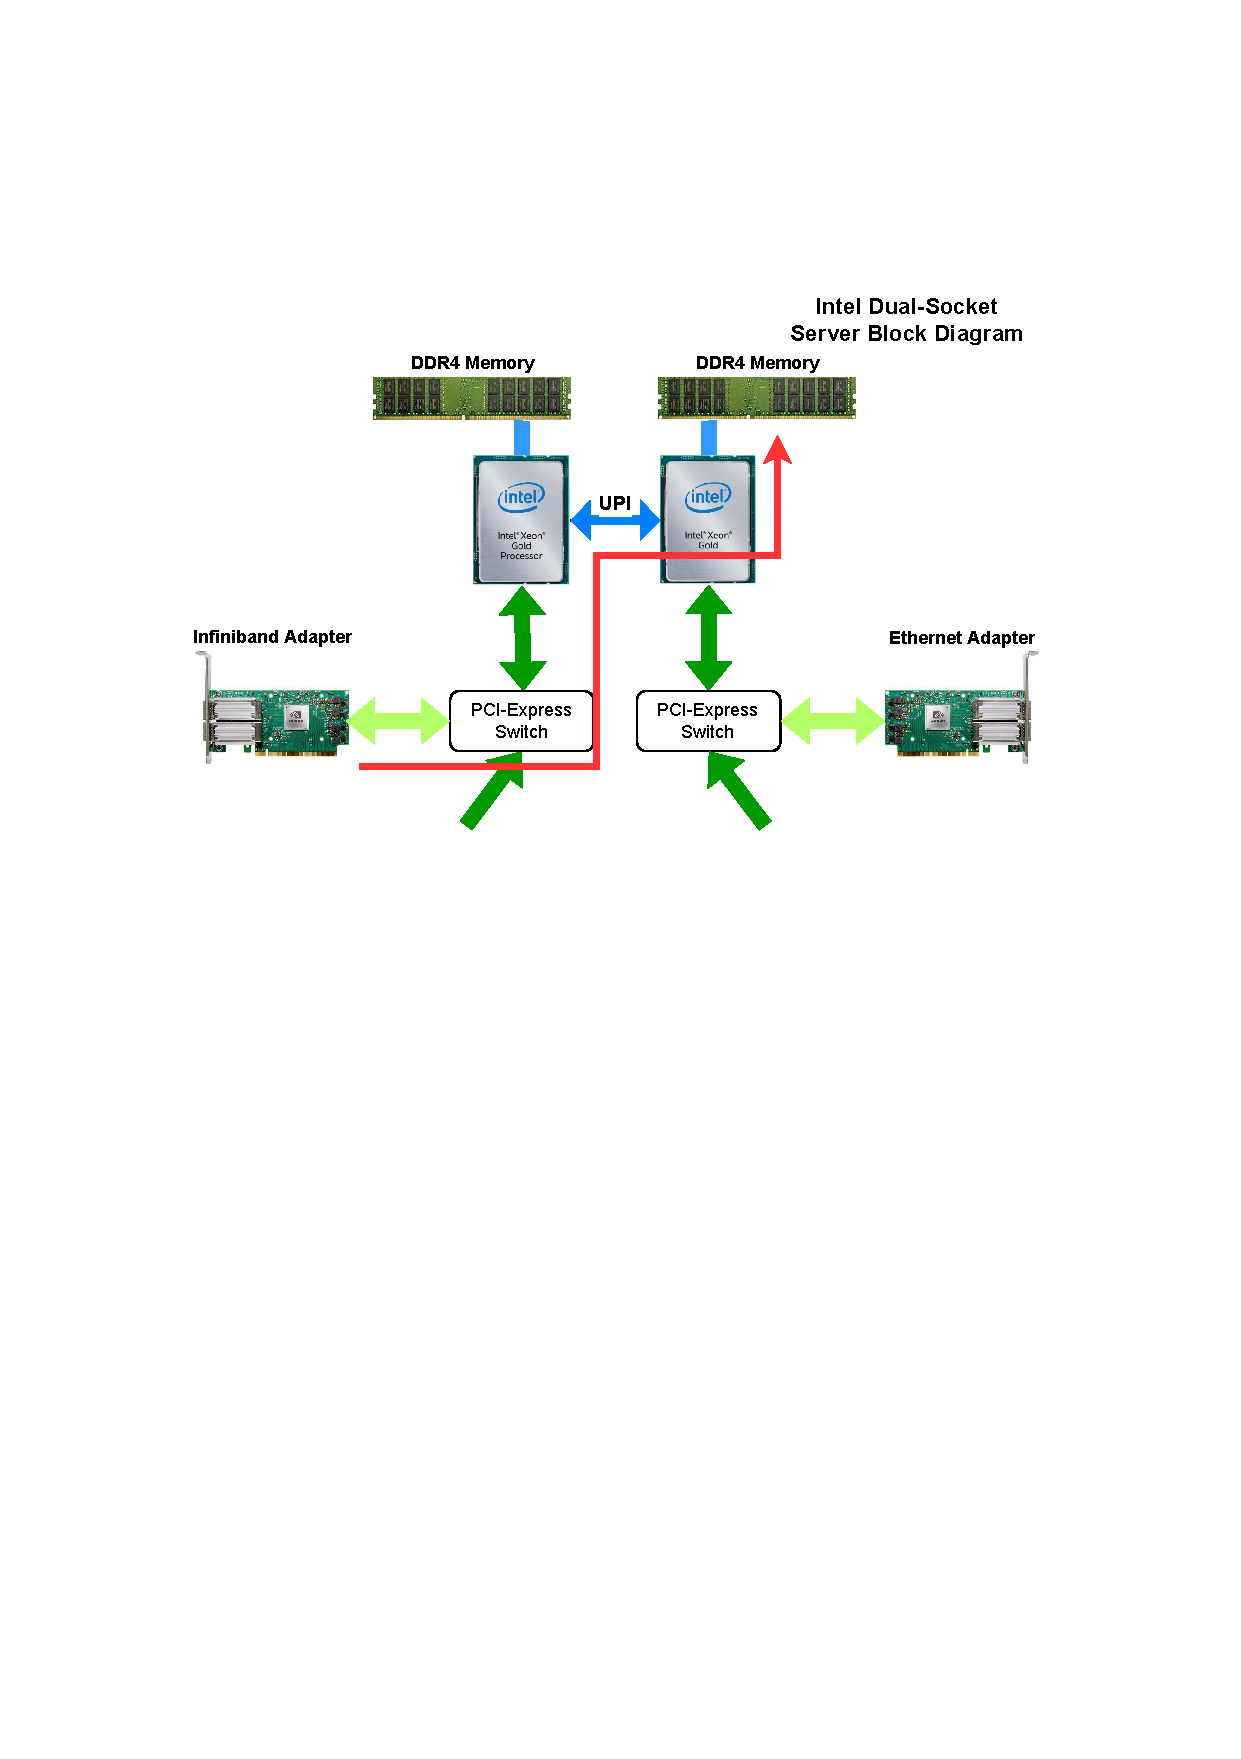
\includegraphics[width=0.8\textwidth]{image/chap04/server_block.pdf}
	\caption{天河CPU服务器硬件拓扑}
	\label{fig:server_block}
\end{figure}

需要注意的是,以太网卡和IB网卡分别挂在两个CPU的PCIe Switch上,因而IB网卡只有在访问本NUMA节点的一半内存时拥有最佳性能——而访问远离它的CPU所控制的一半内存将会有
较大的性能损耗(\autoref{fig:server_block}中\textit{红色访存路线})。这一特性对基于RDMA的网络通信性能有明显的影响,因此在实验中需要相应调整运行配置。

\subsection{软件环境简介}

\autoref{tab:software_config}展示了本章节各性能测试所运行的软件环境。操作系统一栏展示了天河高性能集群使用的Linux操作系统版本;软件依赖指的是成功编译出可正常执行
的Plasma程序所需要的前置软件;测试软件则表示为了编译基准测试程序、运行测试程序所需要的前置软件。所有软件均使用包管理器spack\cite{gamblin2015spack}安装和管理,
软件名后的数字串表示这些软件在测试时使用的版本。

\begin{table}[h]
    \centering
    \caption{天河CPU服务器软件环境}
    \begin{tabular}{*{3}{c}}
        \toprule
        软件类型 & 软件名称  & 作用描述 \\
        \midrule
        操作系统 & CentOS Linux 7 & Linux内核版本3.10.0-957.el7.x86\_64 \\
        \midrule
        包管理器 & spack@0.16.3 & 安装和管理下述软件依赖 \\
        \midrule
        \multirow{3}{*}{软件依赖} & Redis@3.2.3 & \makecell{Redis服务器存放对象在Plasma集群的分布 \\ ae事件循环库驱动Plasma进程} \\
    	 & \makecell{uthash \\ utlist \\ utarray \\ utstring}@2.0.1 & \makecell{基于宏的C语言头文件库,\\ 封装了哈希表等高级数据结构} \\
		 & gcc@9.3.0 & 编译Redis和Plasma \\
        \midrule
    	\multirow{2}{*}{测试软件} & openmpi@4.1.1 & 编译基于MPI的多节点性能测试 \\
		& hwloc@2.5.0 & 查看服务器的NUMA拓扑结构 \\
		& numactl@2.0.14 & 控制MPI进程在NUMA架构下的绑核运行 \\
        \bottomrule
    \end{tabular}
    \label{tab:software_config}
\end{table}

\section{NUMA架构下的Plasma存储测试}

\textbf{跨NUMA节点访存对性能测试的影响:}上一章节中提到了天河高性能集群存在的NUMA访问架构。IB网卡在NUMA架构中,对“远端”CPU所管理的内存发起内存访问需要通过两个CPU之间的UPI互联(The Intel Ultra Path Interconnect,\autoref{fig:server_block}中间\textit{蓝色连接}),
因而无法获得最优的访存延迟和带宽,对Plasma本地存储的性能产生较大的不利影响。由于Plasma传输数据前首先会(在发送端)访问或者(在接收端)创建内存对象,因而会进一步影响Plasma跨节点数据传输的延迟和吞吐能力。
所以,为了获得最佳的传输测试结果,我们将首先通过简单的绑核以优化Plasma的本地存储性能。

在天河高性能服务器中,通过hwloc软件提供的lstopo命令可以查看IB网卡在服务器NUMA架构中所处在的位置:以太网卡挂载在NUMA节点0上,而IB网卡挂载在NUMA节点1上。
这样,我们能通过numactl命令限制plasma\_store和plasma\_manager进程运行在NUMA节点1,从而避免IB网卡的跨NUMA节点访存。

\textbf{绑核性能测试:}为了展示绑核对访存性能的影响,我们分别在绑核与未绑核的情况下测试了Plasma本地存储操作的性能,同时也对Redis进行测试作为参考。结果如\autoref{fig:numa}所示。很显然,不论是本地读还是本地写
使用绑核操作后Plasma的程序性能都有了相当明显的提升:可以看到,在写入较小对象时,绑核的Plasma进程可以获得1.5倍的吞吐能力;不过,绑核运行时的写入性能随着数据增大逐渐下降,
最后和不绑核时持平。在读取和删除对象操作上,绑核在所有数据大小上都有显著的优化效果,其中读取操作的吞吐率增加到原来的至多1.55倍,删除操作的吞吐率增加到原来的至多5倍。

\begin{figure}[h]
    \begin{subfigure}{0.49\textwidth}
        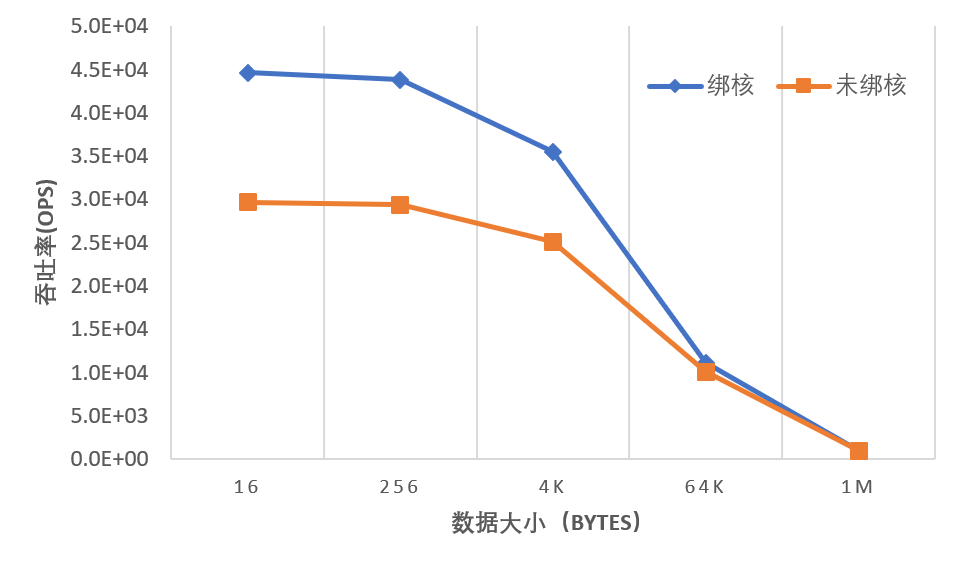
\includegraphics[width=\textwidth]{image/chap04/put.png}
        \caption{Put}
    \end{subfigure}
    \begin{subfigure}{0.49\textwidth}
        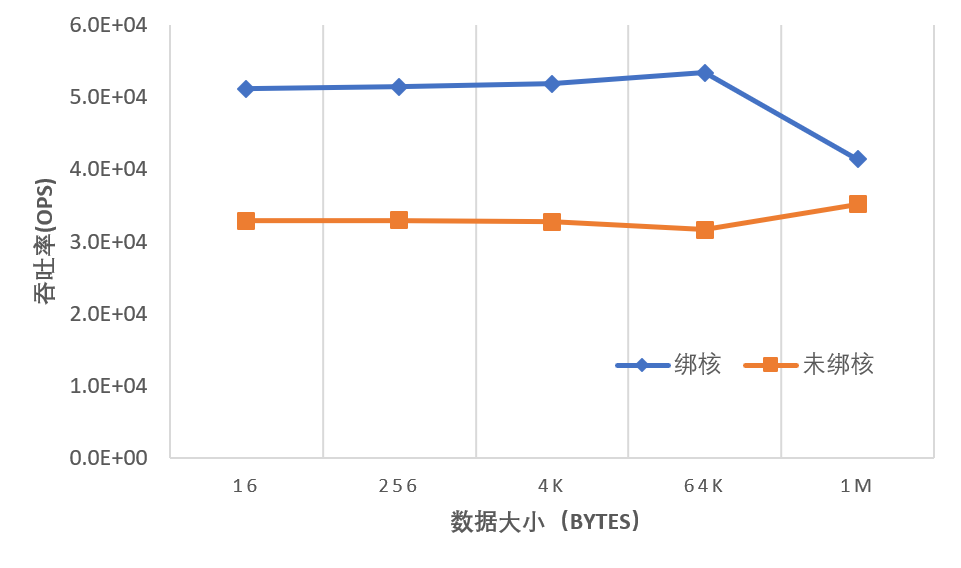
\includegraphics[width=\textwidth]{image/chap04/get.png}
        \caption{Get}
    \end{subfigure}
	\\
	\centering
    \begin{subfigure}{0.5\textwidth}
        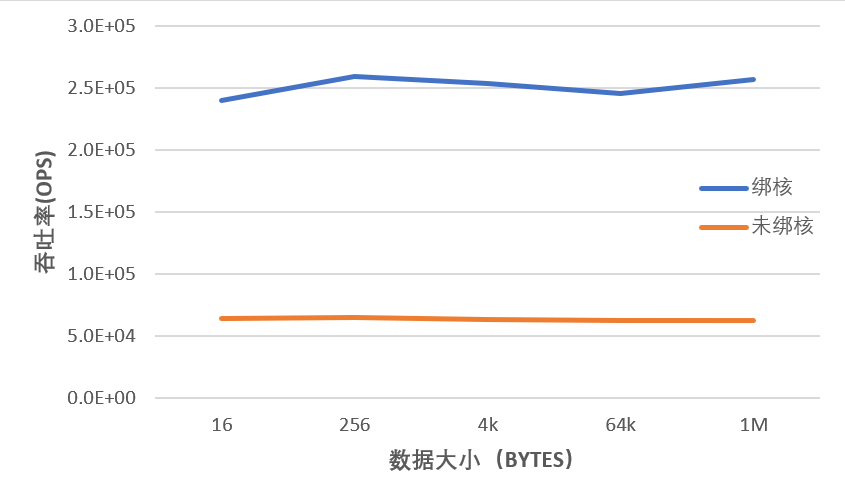
\includegraphics[width=\textwidth]{image/chap04/del.png}
        \caption{Delete}
    \end{subfigure}
    \caption{绑核对Plasma常见操作吞吐率的影响}
    \label{fig:numa}
\end{figure}

与之相比,绑核并不能给Redis带来更强大的吞吐能力——不论是否绑核,Redis在三种常见操作上具有相近的吞吐能力;且在读取/删除操作中,Plasma性能显著更优。
这种区别很有可能是Redis和Plasma传输数据的实现方式不同而导致的:
\begin{itemize}
    \item 如\autoref{sec:plasma_arch}所述,Plasma使用mmap机制获取对象地址后,使用用户态内存拷贝(如memcpy)进行数据读写。
    \item Redis使用的是TCP环回地址(127.0.0.1)向服务器读写数据。
\end{itemize}
Redis在访存上更依赖于操作系统,因此控制Redis进程的NUMA绑核并不会得到明显的性能提升。

由于本地访存的延迟大大降低,且Plasma对象传输过程包括了本地访存操作,因此绑核情况下的多节点传输测试更能够体现出基于RDMA的网络协议在传输性能上的优势。
在之后的性能测试中,基于套接字以及RDMA的传输协议都将以绑核状态运行。

\section{Plasma网络协议测试}

针对Plasma通过以太网络传输数据所导致的性能瓶颈,我们设计了原生支持RDMA通信机制的数据传输协议。针对可能出现的小对象,我们设计了使用预注册缓冲区的双边通信协议;并且,针对可能出现的大对象,
设计了具有完全零拷贝特性的单边传输协议。因此,优化的Plasma通过混合两种机制,能在不同大小的数据都取得较好的吞吐能力。在Plasma优化实现的性能测试中,我们将测试基于IPoIB的套接字、RDMA双边通信以及单边通信在各个数据大小
上的传输性能,一方面验证RDMA机制在性能上的优越性,另一方面可以确定混合机制的关键决策阈值,从而获得最佳的综合性能。

\textbf{性能测试案例的实现:}我们实现了基于MPI编程范式的多进程网络性能测试。该测试能够在一次运行中对Plasma内存存储的主要操作(本地创建/读取/删除和远程读取)进行性能测量。
该测试采用主-从架构,能够支持任意多从进程并发传输的测试。其流程如下所示:

\begin{enumerate}
	\item (0号)主进程阻塞在MPI\_Barrier处,等待(编号为正整数的)从进程创建数据对象。
	\item 其他进程创建一批数据对象。如果进程编号为N-1,测试Plasma本地操作的性能并输出到日志。
	\item 所有进程在MPI\_Barrier处同步。之后,主进程通过MPI\_Gather接口,从其他MPI进程处汇集所有内存对象的标识符。
	\item 主进程以随机顺序向其他进程处发送plasma\_fetch请求,拉取所有数据对象。
\end{enumerate}

\textbf{小对象传输性能:}在天河高性能集群上,我们对N=2,即点对点拉取数据的情况进行性能测试。如\autoref{fig:small}所示,基于双边通信(IB Send/Recv)的传输协议在16K字节范围内的具有最好的传输性能:协议在该数据范围内的传输延迟,
相较基于IPoIB的套接字协议和使用单边通信(IB Read)的协议,均有20微秒的延迟优势。在这一大小范围内,基于IPoIB的套接字协议和使用单边通信的传输协议性能相当——因此后者同样对双边通信协议具有显著的性能差距。这一结果验证了
我们在\autoref{cha:implementation}中的性能分析:即在较小数据的传输中,使用预注册的内存缓冲区和一次用户态的内存拷贝,相比重复注册内存缓冲区具有更小的时间开销,因而是更好的策略。

\begin{figure}[h]
	\centering
	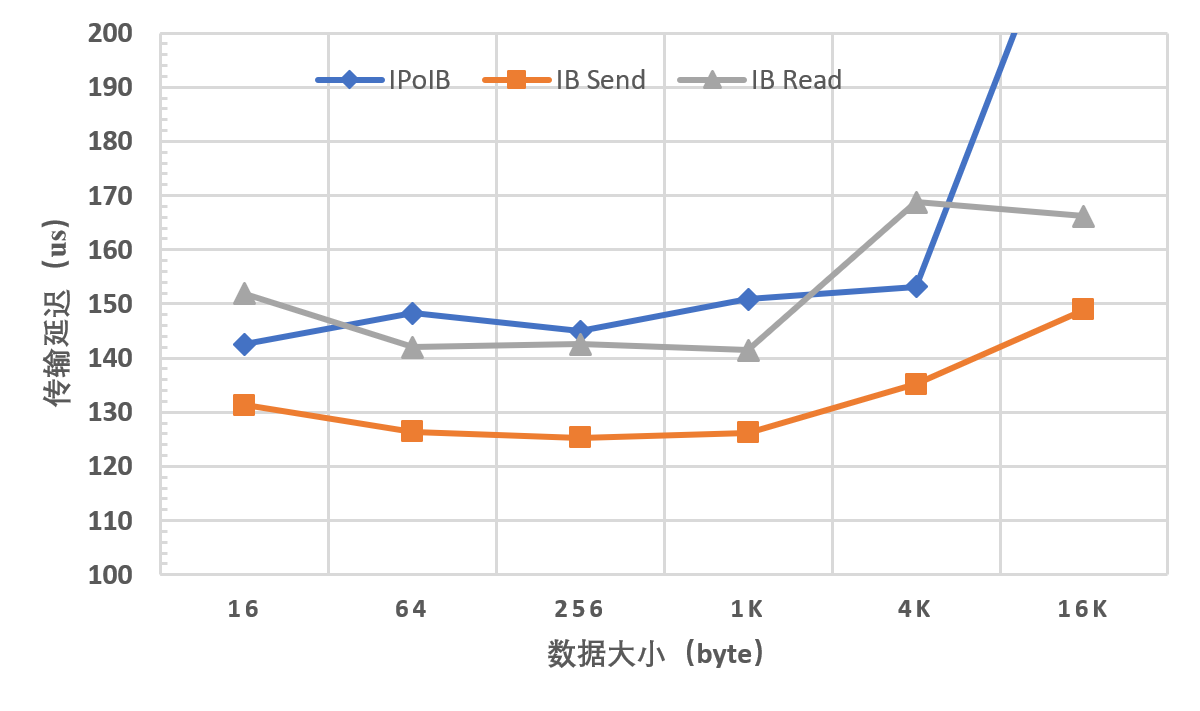
\includegraphics[width=0.9\textwidth]{image/chap04/small.png}
	\caption{三种机制在小对象上的传输延迟}
	\label{fig:small}
\end{figure}

\textbf{大对象传输性能:}并且,上述性能对比在大于16K字节的数据传输中得到了相反的结果,进一步验证了我们对实现的分析。如\autoref{fig:big}所示,原Plasma实现采用的基于IPoIB支持的套接字协议,在每次传输的对象大小大于4K时传输延迟开始快速上升。与之相比的是,随着数据量逐渐增加,使用RDMA机制的传输表现出了更好的扩展性:
不论是基于RDMA的双边通信还是单边通信的传输协议,都表现出了明显的性能优势。使用套接字协议传输1M字节大小的内存对象,RDMA双边传输协议可以在相似时间内传输四倍大小的数据量。进一步,在这一大小范围内,使用RDMA单边读的传输协议,对使用双边通信的传输协议也具有明显的性能优势。
当对象大小大于16K字节时,前者表现出更优的传输延迟,并且该优势随着数据量增大而显著增大——在4M字节的对象传输中,使用单边RDMA操作能将吞吐率再增加一倍。在这一数据大小上,RDMA的较优通信方案表现出了7倍于原实现的传输性能。

\begin{figure}[h]
	\centering
	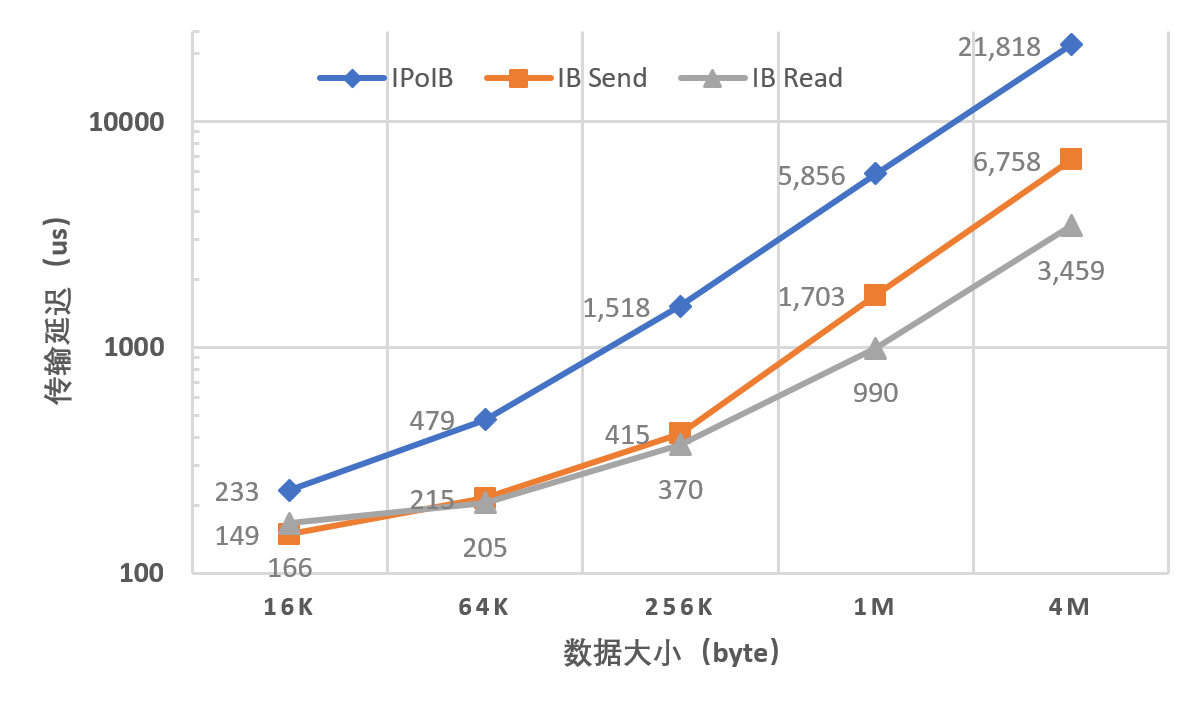
\includegraphics[width=0.9\textwidth]{image/chap04/big.png}
	\caption{三种机制在大对象上的传输延迟}
	\label{fig:big}
\end{figure}

\textbf{混合机制的选择:}上述性能测试在各个常见的数据范围内,展示了原生RDMA机制对传统套接字通信的性能优势。并且,在\autoref{cha:implementation}中我们实现了两种通信协议,并分析了它们的预期性能特征——这一讨论在实验中也得到了充分验证。为了让Plasma能在各个数据范围内充分利用RDMA机制的性能优势,
我们通过观察实验数据,选择常量IB\_READ\_MIN\_SIZE的值为32KB。以该常量值为分界线,当对象大小小于该值时使用双边传输协议,反之使用单边传输协议。此时,我们能够将两种机制的性能特征简单而有效地结合起来,从而达到Plasma实现的最大优化。值得注意的是,最优的参数应当随着CPU、IB网卡、内存等硬件的性能发生变动。
不过,通过我们在本研究中实现的性能测试程序,确定最优的策略应该是容易的。

\textbf{与Redis对比:}在确认了Plasma最佳的混合传输策略之后,我们可以将优化的Plasma实现和Redis作性能对比。两者传输各个大小数据的延迟如\autoref{fig:redis_small}和\autoref{fig:redis_big}所示。
和\autoref{sec:bench}不同,经过RDMA传输优化后的Plasma,已经能在常见大小的对象传输上获得比Redis
显著更优的性能。然而还需要强调的是,Plasma在传输测试中所完成的操作,明显要比Redis更多——Plasma每次拉取对象到本地内存中,都会再次创建该对象、分配等大的内存空间、拷贝数据并封存;而Redis在性能测试中并不会这么做。总结来说,这是Plasma为了支持Ray分布式缓存、分布式访问所需的额外代价。
然而,通过借助RDMA的硬件优势,我们优化了Plasma内存存储的传输机制,使其同时拥有了如下技术优势:

\begin{enumerate}
    \item 支撑分布式计算框架Ray的集群内存管理,相比Redis数据库,Plasma是分布式、可扩展的。
    \item 即便是实现了分布式内存对象存储,Plasma在任意单节点上的性能仍然显著地优于Redis数据库。
\end{enumerate}

\begin{figure}[h]
	\centering
	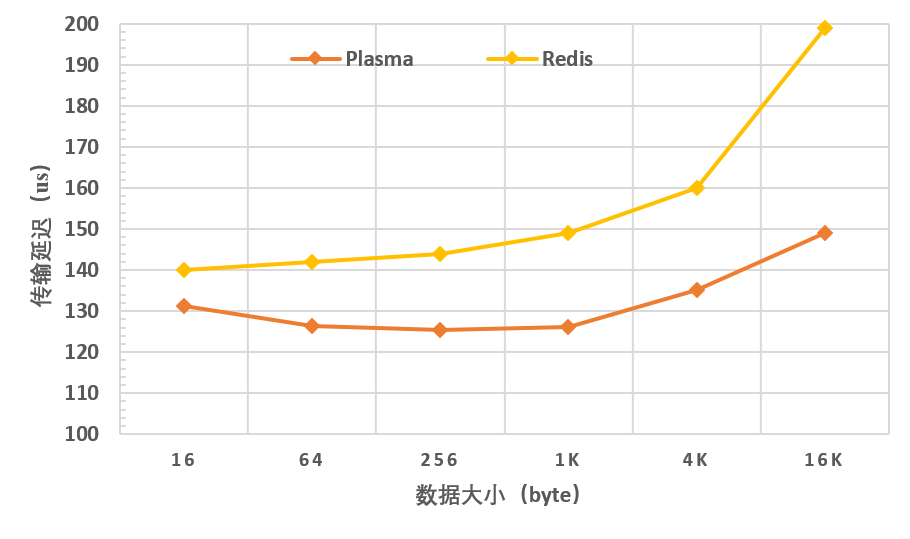
\includegraphics[width=0.9\textwidth]{image/chap04/redis_small.png}
	\caption{Redis和Plasma在小对象上的传输延迟}
	\label{fig:redis_small}
\end{figure}

\begin{figure}[h]
	\centering
	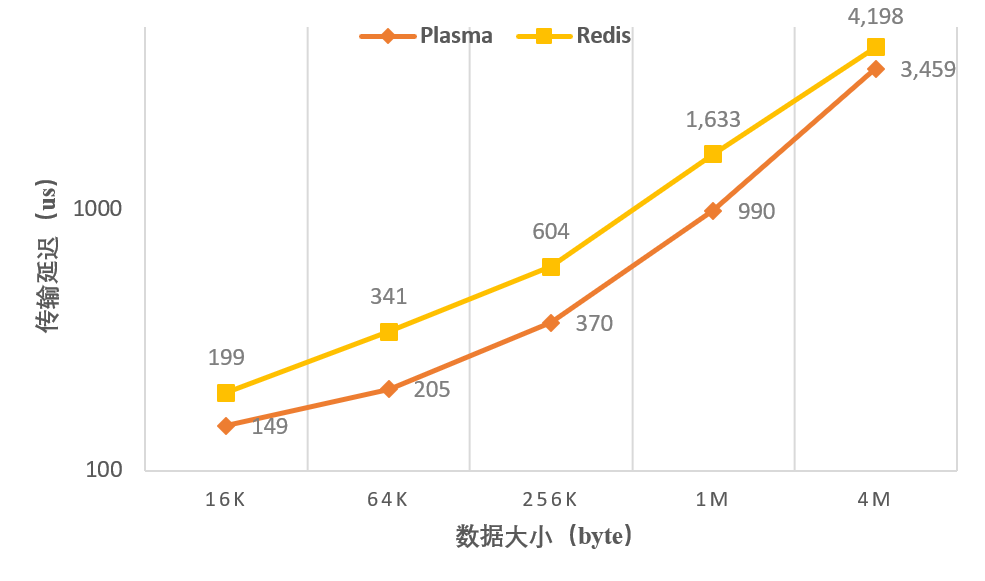
\includegraphics[width=0.9\textwidth]{image/chap04/redis_big.png}
	\caption{Redis和Plasma在大对象上的传输延迟}
	\label{fig:redis_big}
\end{figure}